% !TEX program = arara
% arara: pdflatex
% arara: biber
% arara: pdflatex
% arara: pdflatex
% arara: clean: { files: [ Bericht.out ] }
% arara: clean: { files: [ Bericht.aux, Bericht.bbl ] }
% arara: clean: { files: [ Bericht.bcf, Bericht.blg ] }
% arara: clean: { files: [ Bericht.log, Bericht.run.xml ] }
% arara: clean: { files: [ Bericht.toc, Bericht-blx.bib ] }
% 

\documentclass{Bericht}
\usepackage{todonotes}
\usepackage[utf8]{inputenc}
\usepackage{hyperref} % http://ctan.org/pkg/hyperref
\usepackage{graphicx}
%\usepackage[ngerman]{babel} % deutsche Silbentrennung
\usepackage{float}
\hypersetup{
	colorlinks = true,
	linkcolor  = black
}

\begin{document}

\maketitle

% % % % %

\tableofcontents
\clearpage

\section{Einleitung}
	\todo[inline]{Autor: Kim}
	Das Thema Zeitempfinden spielt in unserer modernisierten Gesellschaft eine immer wichtiger werdende Rolle. Zwischen Arbeit, Freizeit und Familie ist es wichtig, seine Zeit ganz genau zu planen und jede freie Minute auszunutzen. Aufgrund des Wissens, dass die arbeitende Bevölkerung sich an bestimmte Zeitregeln hält und versucht den Alltag optimal zu managen und unter Betrachtung der zunehmenden Relevanz von Zeitmanagement und Zeitsparen, richteten wir unsere Forschung auf das Thema der Zeitmanpulation. Zunächst gilt zu definieren, was Zeit überhaupt ist: „Zeit ist das Nacheinander von Zuständen und Ereignissen, die erlebbar und messbar sind. Sie ist eine physikalische Größe für die Vergänglichkeit und Veränderungen“. (\underline{http://definition-online.de/zeit/})
	\par
	In unserer Lebenswelt gibt es bestimmte Zeitgeber, von der Uhrzeit selber einmal abgesehen, die uns Hinweise geben, wieviel Zeit vergangen ist. Für uns galt es nun herauszufinden, ob es möglich ist, anhand gängiger Zeitgeber, die jeden einzelnen Menschen seit der Geburt täglich begleiten, eine Manipulation des Zeitempfindens auszulösen. Anhand unserer Forschungsfrage: „Kann man das Zeitempfinden in der Virtuellen Welt durch bestimmte Zeitgeber manipulieren“ erschufen wir eine Virtuelle Welt, durch die unsere späteren Probanden mit Hilfe einer VR-Brille manipulierte Zeitgeber erlebten. 
	\par
	 Wir legten einen weiteren Fokus unserer Arbeit auf die Zeitschätzung. Jeder Proband wurde gebeten, vor und nach dem Befinden in der Virtuellen Welt eine bestimmte Sekundenanzahl abzuschätzen, ohne auf Hilfsmittel zuzugreifen, wie beispielsweise eine Armbanduhr. Auf diese Weise wollen wir herausfinden, ob sich die Zeitschätzung vor dem Befinden in der Virtuellen Welt von der Zeitschätzung nach dem Befinden in der Virtuellen Welt unterscheidet.
Dieser Bericht führt über die Ideenfindung unserer Forschungsschwerpunktes zu unseren Hypothesen. Nach der technischen und kreativen Umsetzung unseres Experiments und unserer virtuellen Welt wird der detaillierte Ablauf des Experiments beschrieben. Im Zweiten Teil- dem empirischen Teil- folgen die Auswertungen, Ergebnisse und Interpretationen und der Bezug zu unseren Hypothesen. Am Ende des Berichts gibt es einen kurzen Überblick über die Zusammenarbeit der Forschungsgruppe und ein abschließendes Fazit. 
	\par
	\textit{„Zeit ist das, was man an der Uhr abliest.“ (Albert Einstein)}
	\par
	Ob diese Definition wirklich ausreicht, oder ob es andere wichtige Zeitgeber gibt, die das menschliche Zeitempfinden vorgeben, gilt es herauszufinden. 

\section{Ideenfindung und Hypothese}
	\todo[inline]{Autor: Berna}
	Protokoll für das Meeting am Montag, den 24.04.2017:
Mit der Unterstützung unseres Dozenten haben wir eine grobe Vorstellung davon bekommen, wie unser Projekt aussehen könnte. Um die Erwartungen an dieses Projekt und die Art und Weise wie es durchgeführt werden soll abzudecken, haben wir mit Hilfe des Brainstormings Ideen gesammelt. Dabei war es neben der Ideensammlung wichtig, utopische Vorstellungen nicht sofort zu verwerfen. Durch die Virtual Reality wollten wir beispielsweise Probanden dazu bringen, gegen ihre Phobie, wie die Höhenangst oder die Angst vor Spinnen anzukämpfen. Außerdem wollten wir versuchen, die Probanden in einen „anderen“ Körper zu stecken. Damit ist ein anderes Geschlecht, die Hautfarbe oder ähnliches gemeint, welches mit einem Körper – Tracker realisiert werden könnte. Hierbei lag der Fokus besonders darauf, ob sich die Probanden auch wirklich in einen dieser Körper hineinversetzen könnten beziehungsweise ob sich das Gehirn dem anpasst. Darüber hinaus hatten wir einen Einfall, dass Probanden in der Virtual Reality einen Superhelden verkörpern könnten, denn laut Studien sollen sie durch diese Konfrontation sozialisierter werden. Natürlich stellte sich demzufolge die Frage, was passieren würde, wenn man einen Probanden in einen Schurken transformiert. Könnte sich das Verhalten ins Negative auswirken? Eine weitere Idee war, Rollstuhlfahrer mit ihren Gedanken eigene Bewegungen steuern zu lassen. Dieser Blickwinkel ist und war allerdings schwer zu realisieren, da Rollstuhlfahrer als Probanden fungieren müssten. Des Weiteren wäre eine Studie interessant, die aussagt, wie weit Probanden in der Virtual Reality gehen würden. Wären sie bereit, Leute in einem Spiel zu liquidieren? Sollte dieser Fall eintreten, würden bei diesen Probanden die Gehirnschwingungen gemessen werden und Veränderungen oder Unterschiede notiert. Ideen in diese Richtung wurden aber letztendlich verworfen, da es nicht der Ethik der Wissenschaft entspricht. Eine weitere Idee war, einen bewegenden, emotional ansprechenden Film vor sowie nach dem Befinden in der Virtual Reality abzuspielen, um zu prüfen, ob sich der Proband nun anders verhält, mitfühlender, sensibler, hilfsbereiter oder ähnliches ist als vorher. Für die spätere Auswertung sollten einige Werte gemessen und festgehalten werden, wie zum Beispiel die Feuchtigkeit der Haut, der Herzschlag oder die Gehirnströme.
\par
Nachdem wir die oben beschriebenen Ideen gesammelt und festgehalten hatten, ging es daraufhin um die Recherche für mehr Input und dem Abgleich, ob schon vorhandene Experimente in die Richtung durchgeführt wurden. Während dieses Vorgehens kamen uns noch weitere Gedanken. Einer davon war, den Probanden mit Hilfe eines Pinsels am Oberkörper zu streicheln. An dieser Stelle wird dann in der Virtual Reality Welt genau dieser Pinsel zu sehen sein, welcher ihn streichelt. Passt sich das Gehirn dem an? Der Grundgedanke dabei war, wie sie in einer schnelleren oder langsameren Welt interagieren. Gibt es beispielsweise Unterschiede im Bewegungsablauf oder in der Reaktionsfähigkeit? Dazu wäre es wichtig, Reaktionstests durchzuführen, Wettrennen, das Laufen in der Virtual Reality, Bälle zu fangen, Sachen zu sammeln, oder das Laufband schneller beziehungsweise langsamer für die Haptik einzustellen. Um die Welt so realistisch wie möglich dazustellen, sollte mit Hand – Trackern gearbeitet und zusätzlich die Illusion vom selber sprechen erschaffen werden. Dafür wird ein Spiegel in die Virtual Reality eingebaut, um den Avatar sprechen zu sehen. Außerdem sollte es einen Vergleich zwischen Kindern und Erwachsenen geben mit der Frage: „Gibt es Unterschiede bei Kindern oder Erwachsenen, welches die Reaktionsfähigkeit nach dem Virtual Reality Experiment betrifft?“. Durch das Einbeziehen aller Ideen haben wir uns schlussendlich auf folgende Forschungsfrage geeinigt: „Wie verändert sich das Zeitempfinden in der realen Welt auf den Avatar durch einwirkende Zeitraffung bzw. Zeitdehnung in der Virtual Reality?“. Unser Fokus liegt unter Beachtung all dieser Dinge auf dem Zeitempfinden des Probanden. Mit dem Ausbau dieser Idee hatten wir einige Vorstellungen wie die Virtual Reality aufgebaut werden sollte. Wir wollten einige Situationen bieten, wie zum Beispiel: durch die Stadt laufen, eine Welt mit Uhren, Autos, Fahrräder, Tiere, andere Menschen, Bäume, Heißluftballons und die Interaktion mit Probanden, die Aufgaben erledigen sollen. Aufgaben die das Flyer verteilen beinhalten, laufen, Bälle fangen oder im Schaufenster mit sich reden / sich sehen (‘body transfer illusion‘).
\par
Es ist wichtig zu erwähnen, dass es drei VR – Welten gibt. Eine langsame, eine schnelle und eine mit einer normalen Zeiteinheit in der die Probanden interagieren müssen. Pro Kategorie sollte es eine aktive und eine passive Interaktion geben. Probanden in der langsamen Welt erledigen Aufgaben, die einen einfachen Schweregrad kennzeichnen, wie das Erkunden der Gegend. Des Weiteren hatten wir die Idee, das Experiment an einem Strand mit unterschiedlichen Sonnenbewegungen durchzuführen. Es sollte außerdem darauf geachtet werden, dass in der schnellen Welt die Sonne schneller untergeht, sprich, dass die Zeitabläufe den Welten angepasst werden.
\par
Schlussendlich haben wir uns noch einmal mit unserem Dozenten zusammengesetzt und über unsere bestehende Forschungsfrage nachgedacht. Dabei sind wir zu dem Entschluss gekommen, dass zu viele Tasks das Experiment in die Länge ziehen. Aus diesem Grund wurde das Konzept noch einmal überarbeitet, was zur Folge hatte, dass sich die Forschungsfrage änderte. Die aktuelle lautet nun: „Kann man das Zeitempfinden in der Virtuellen Welt durch bestimmte Zeitgeber manipulieren?“

%\section{Hypothese}
	%\todo[inline]{Autor: Berna}
	%	Hier steht die Hypothese.

\clearpage
\section{Verlauf}
	\todo[inline]{Autor: Marvin \& Daniel}
	\subsection{Planung/Recherche} % Marvin
	
		%Erster Kontakt
		Erster Berührungspunkt mit dem Bachelorprojekt ¡Experiment! war für viele Gruppenmitglieder die Vorstellung eben dessen durch Thorsten Kluß am 24.01.2017 an der Hochschule für Künste, bzw. deren Wiederholung am 06.04.2017 an der Universität Bremen. Erweitert wurde der zweite Termin dabei durch eine Führung der Räume des 'Cartesiums', sowie eine Beschreibung der vorangegangen Bachelorprojekte. Hierdurch konnte ein erster Eindruck über die verschiedenen Versuchsaufbauten und ferner der Beschaffenheit unseres Projekts gewonnen werden. An dieser Stelle wurde zunächst eine Recherche-Aufgabe zu vorbereiteten Texten ausgeteilt, welche allein oder in kleineren Gruppen bearbeitet und später präsentiert werden sollte.\\
\\
		%Erwartungen
		Am darauffolgenden Termin wurden uns von den Dozenten (Thorsten Kluß und Jaime Maldonaldo, später zusätzlich Kerstin Bub) alle Erwartungen, sowie Schein- und Arbeitsbedingungen dargelegt.\\
\\
		%Social & Arbeitsweise/Zeiten
		Neben den üblichen 'Kennenlern-Ritualen', wie z.B. dem Herausstellen der eignen Stärken und Schwächen anhand von 'Skill-Profilen', wurden die ersten zwei Wochen der Projektarbeit hauptsächlich für technische Organisation, Planungs- und Recherchezwecke genutzt. Dabei entschied man zunächst, dass ein 'Scrum'-Modell mit geteilter 'Scrum-Master'-Position für das Projektmanagement genutzt werden soll. Anhand der bereits erwähnten Fähigkeitenprofile wurde die Gruppe 7-3 in zwei Teams mit unterschiedlichen Schwerpunkten aufgeteilt('Design' und 'Organisation').\\
		Weiterhin wurde ein umfassender Stundenplan aus den einzelnen Stundenplänen für das restliche Studium jedes Teilnehmers erstellt. Anhand dessen wurden Zeiten an vier Tagen der Woche ermittelt, welche für Treffen der Arbeitsgruppe zum Bachelorprojekt genutzt werden sollten, mit einem zusätzlich Slot am Donnerstag für ein Meeting mit den Dozenten. \\
		Zu Beginn jeden Arbeitstages wurde ein 10-minütiges 'Scrum-Treffen' gehalten, in denen anstehende Aufgaben aus dem Backlog und Probleme besprochen wurden. Diese besonderen Treffen wurden jedoch nie regelmäßig eingehalten, vor allem in späteren, arbeitsintensiveren Phasen nicht.\\
		Ferner wurde für die Protokollführung der Treffen eine feste Reihenfolge angelegt.\\
\\
		%Raum
		Leider war es unseren Dozenten nicht möglich, eine dedizierten Raum für unseren Arbeitsprozesse zu erhalten, weshalb die Treffen je nach Situation im Konferenzraum 4.43 des vierten Stockwerks oder den Räumen 4.12 und 4.16 (ebenfalls vierter Stock) im Cartesium abgehalten worden sind. Um Zugang zu der Etage und diesen Räumen zu gewährleisten, erhielten wir mit einiger Verzögerung jedoch Türchips für das spezielle Schließsystem des Cartesiums.\\
\\
\newpage
		% Tech
		Auch wurden alle technischen Lösungen zur Arbeitsweise in dieser Zeit implementiert. Als zentrale Sammelstelle für sämtliche Dokumente wurde ein Board beim Service 'Trello' genutzt. Dort ließen sich bequem und zugänglich für alle Teilnehmer sämtliche wöchentlichen Sprints sowie der Backlog des Scrum, die Protokolle und der Stundenplan, etc. ablegen. Für schnelle Kommunikation untereinander wurde der Nachrichtendienst 'WhatsApp' genutzt, da diese Applikation bereits auf sämtlichen Endgeräten der Teilnehmer installiert war. Leider wurde dieser Dienst nicht von den Dozenten genutzt und wir verließen uns auf Kommunikation per E-Mail mit diesen, sowie Telefonate in dringenden Fällen.\\
		\begin{figure}[H] % here - top - bottom - page, das ! erzwingt die Position falls möglich
			\centering
			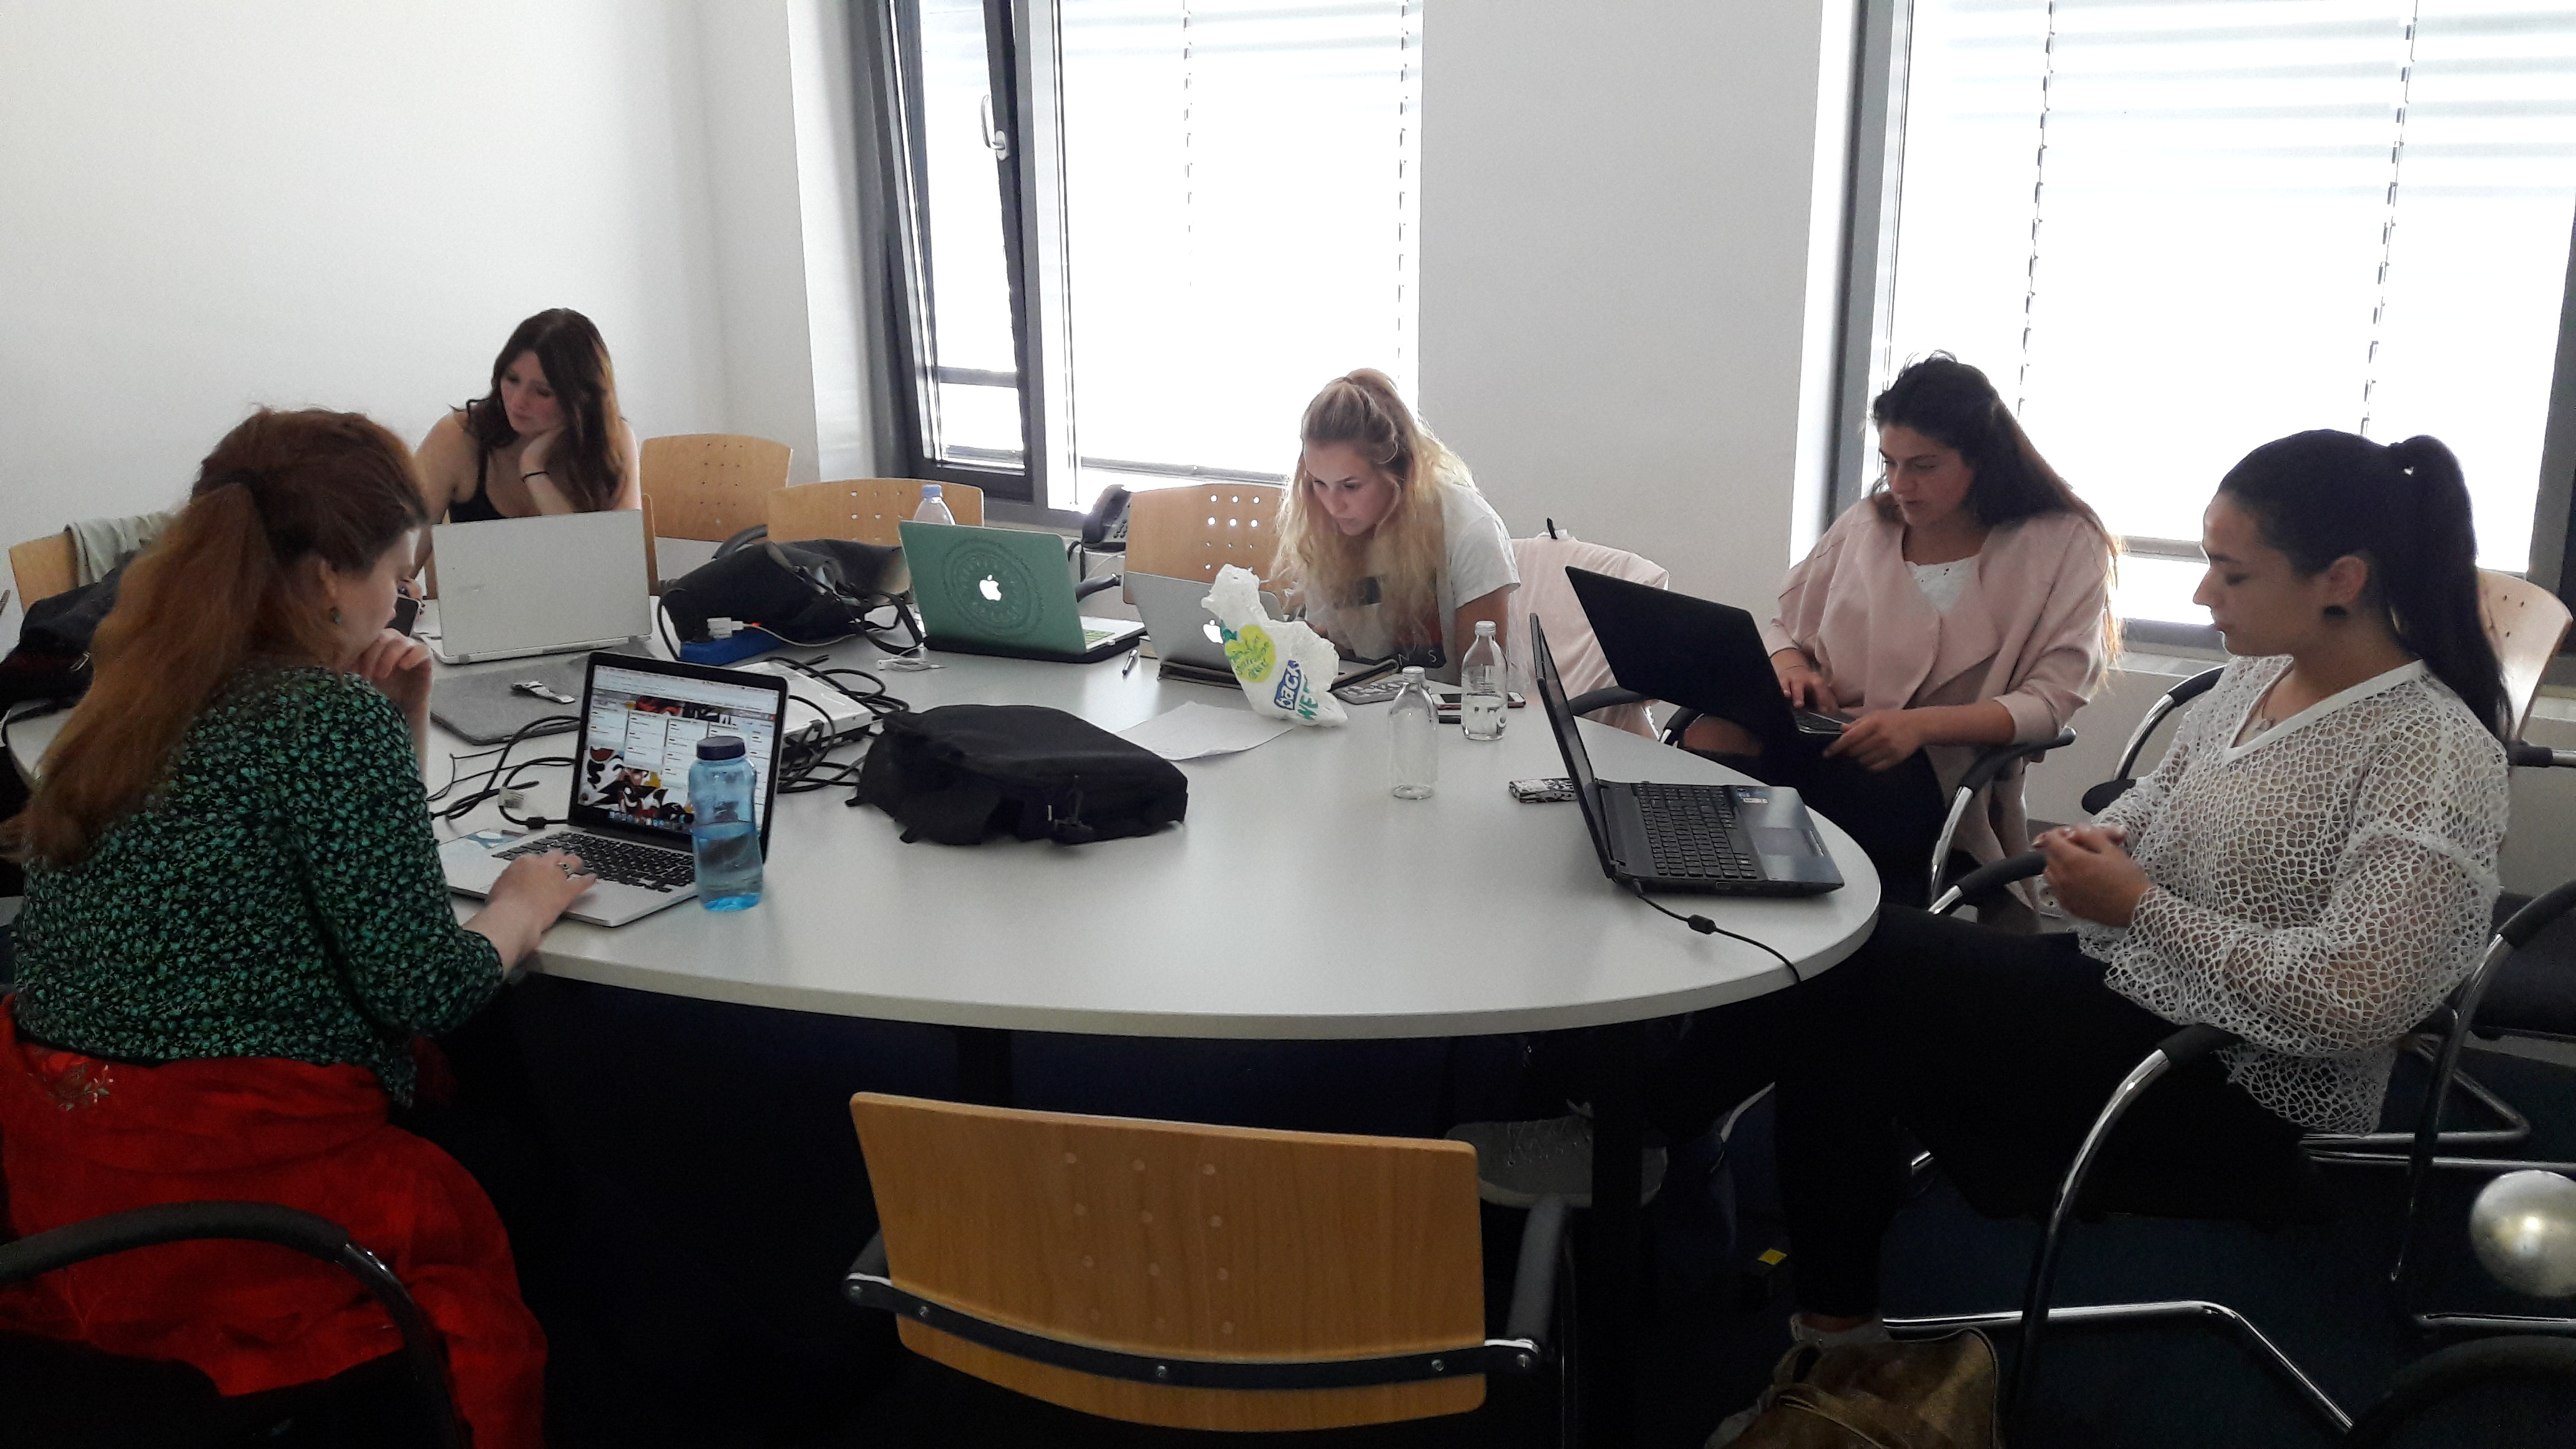
\includegraphics[width=\linewidth, height=\textheight, keepaspectratio]{Bilder/20170518_103125.jpg}
			\caption{Das ¡Experiment!-Team bei der Arbeit}
			\label{img:experiment-team-bei-der-arbeit}
		\end{figure}
		%Recherche
		Die ersten Rechercheleistungen beschäftigten sich hauptsächlich mit wissenschaftlichen Arbeitsweisen, existierenden technischen Möglichkeiten und bereits durchgeführter Forschung. Vollkommen fehlgeleitet und geblendet von technischen Besonderheiten wie dem möglichen Hand-Tracking durch 'LeapMotion' oder der Bewegungsteuerung durch [die Kugel] versuchten wie eine Forschungsfrage passend zu diesen zu entwickeln.\\
		Wie im 'Paragraphen 2: Ideenfindung' beschrieben, dauerte es eine gewisse Zeit bis wir eine konkrete, realisierbare Forschungsfrage zur Manipulation des Zeitempfindens innerhalb der 'Virtual Reality' ausarbeiten konnten. Maßgeblich geholfen hat uns dabei die Grundlagenforschung zur Zeitwahrnehmung in der VR von Gerd Bruder.\\
\\
		%Überschneidung
		Die genauen Spezifikationen an unser Experiment gemäß der Forschungsfrage wurden nach Rücksprache mit den Dozenten immer wieder verändert. Hierdurch entstand viel unbenutzbares Material, da wir überschneidend bereits damit begonnen hatten, 3D-Objekte nach den ersten Anforderungen für unsere Versuchswelt zu erstellen. Dies geschah fälschlicherweise aus dem Versuch heraus, bereits verlorene Zeit aufzuholen, wodurch jedoch nur mehr 'Verschnitt' produziert worden ist, was uns ultimativ uns mehr Zeit gekostet hat.\\
\\
		%Weiterführend
		Wir approximierten, dass sich ab diesem Zeitpunkt unser Projekt in 3 Phasen (Programmierphase, Versuchsphase, Evaluation/Paper) 	unterteilen ließe und legten Deadlines für die einzelnen fest. Im Laufe des Projektes sollten wir jedoch erkennen, wie weit entfernt diese Einschätzungen von der Realität abwichen.

	\subsection{Design} % Daniel
		\todo{methodisches Versuchsdesign}
		Angefangen haben wir mit dem Erstellen von 3D-Objekten. Aus einer Liste mit benötigten Objekten suchte sich jeder aus dem Technikteam einige heraus und begann sie zu designen. Folgende Objekte wurden erstellt, wenn auch nicht alle im finalen Projekt zum Einsatz kamen:
		
		\begin{itemize}
			\setlength{\itemsep}{0em}
			\item Ampel
			\item Autos
			\item Blume
			\item Bäume
			\item Büsche
			\item Garten
			\item Gehsteige
			\item Heißluftballon
			\item Hund
			\item Häuser
			\item Laterne
			\item Menschliche NPCs
			\item Mülleimer
			\item Parkbank
			\item Plakat
			\item Rasenfläche
			\item Reiher
			\item Schaukel
			\item Sonne
			\item Straße
			\item Straßenschilder
			\item Supermarkt
			\item Wolken
			\item Zimmerpflanze (Kaktus)
		\end{itemize}
		
		\begin{figure}[!htbp] % here - top - bottom - page, das ! erzwingt die Position falls möglich
			\centering
			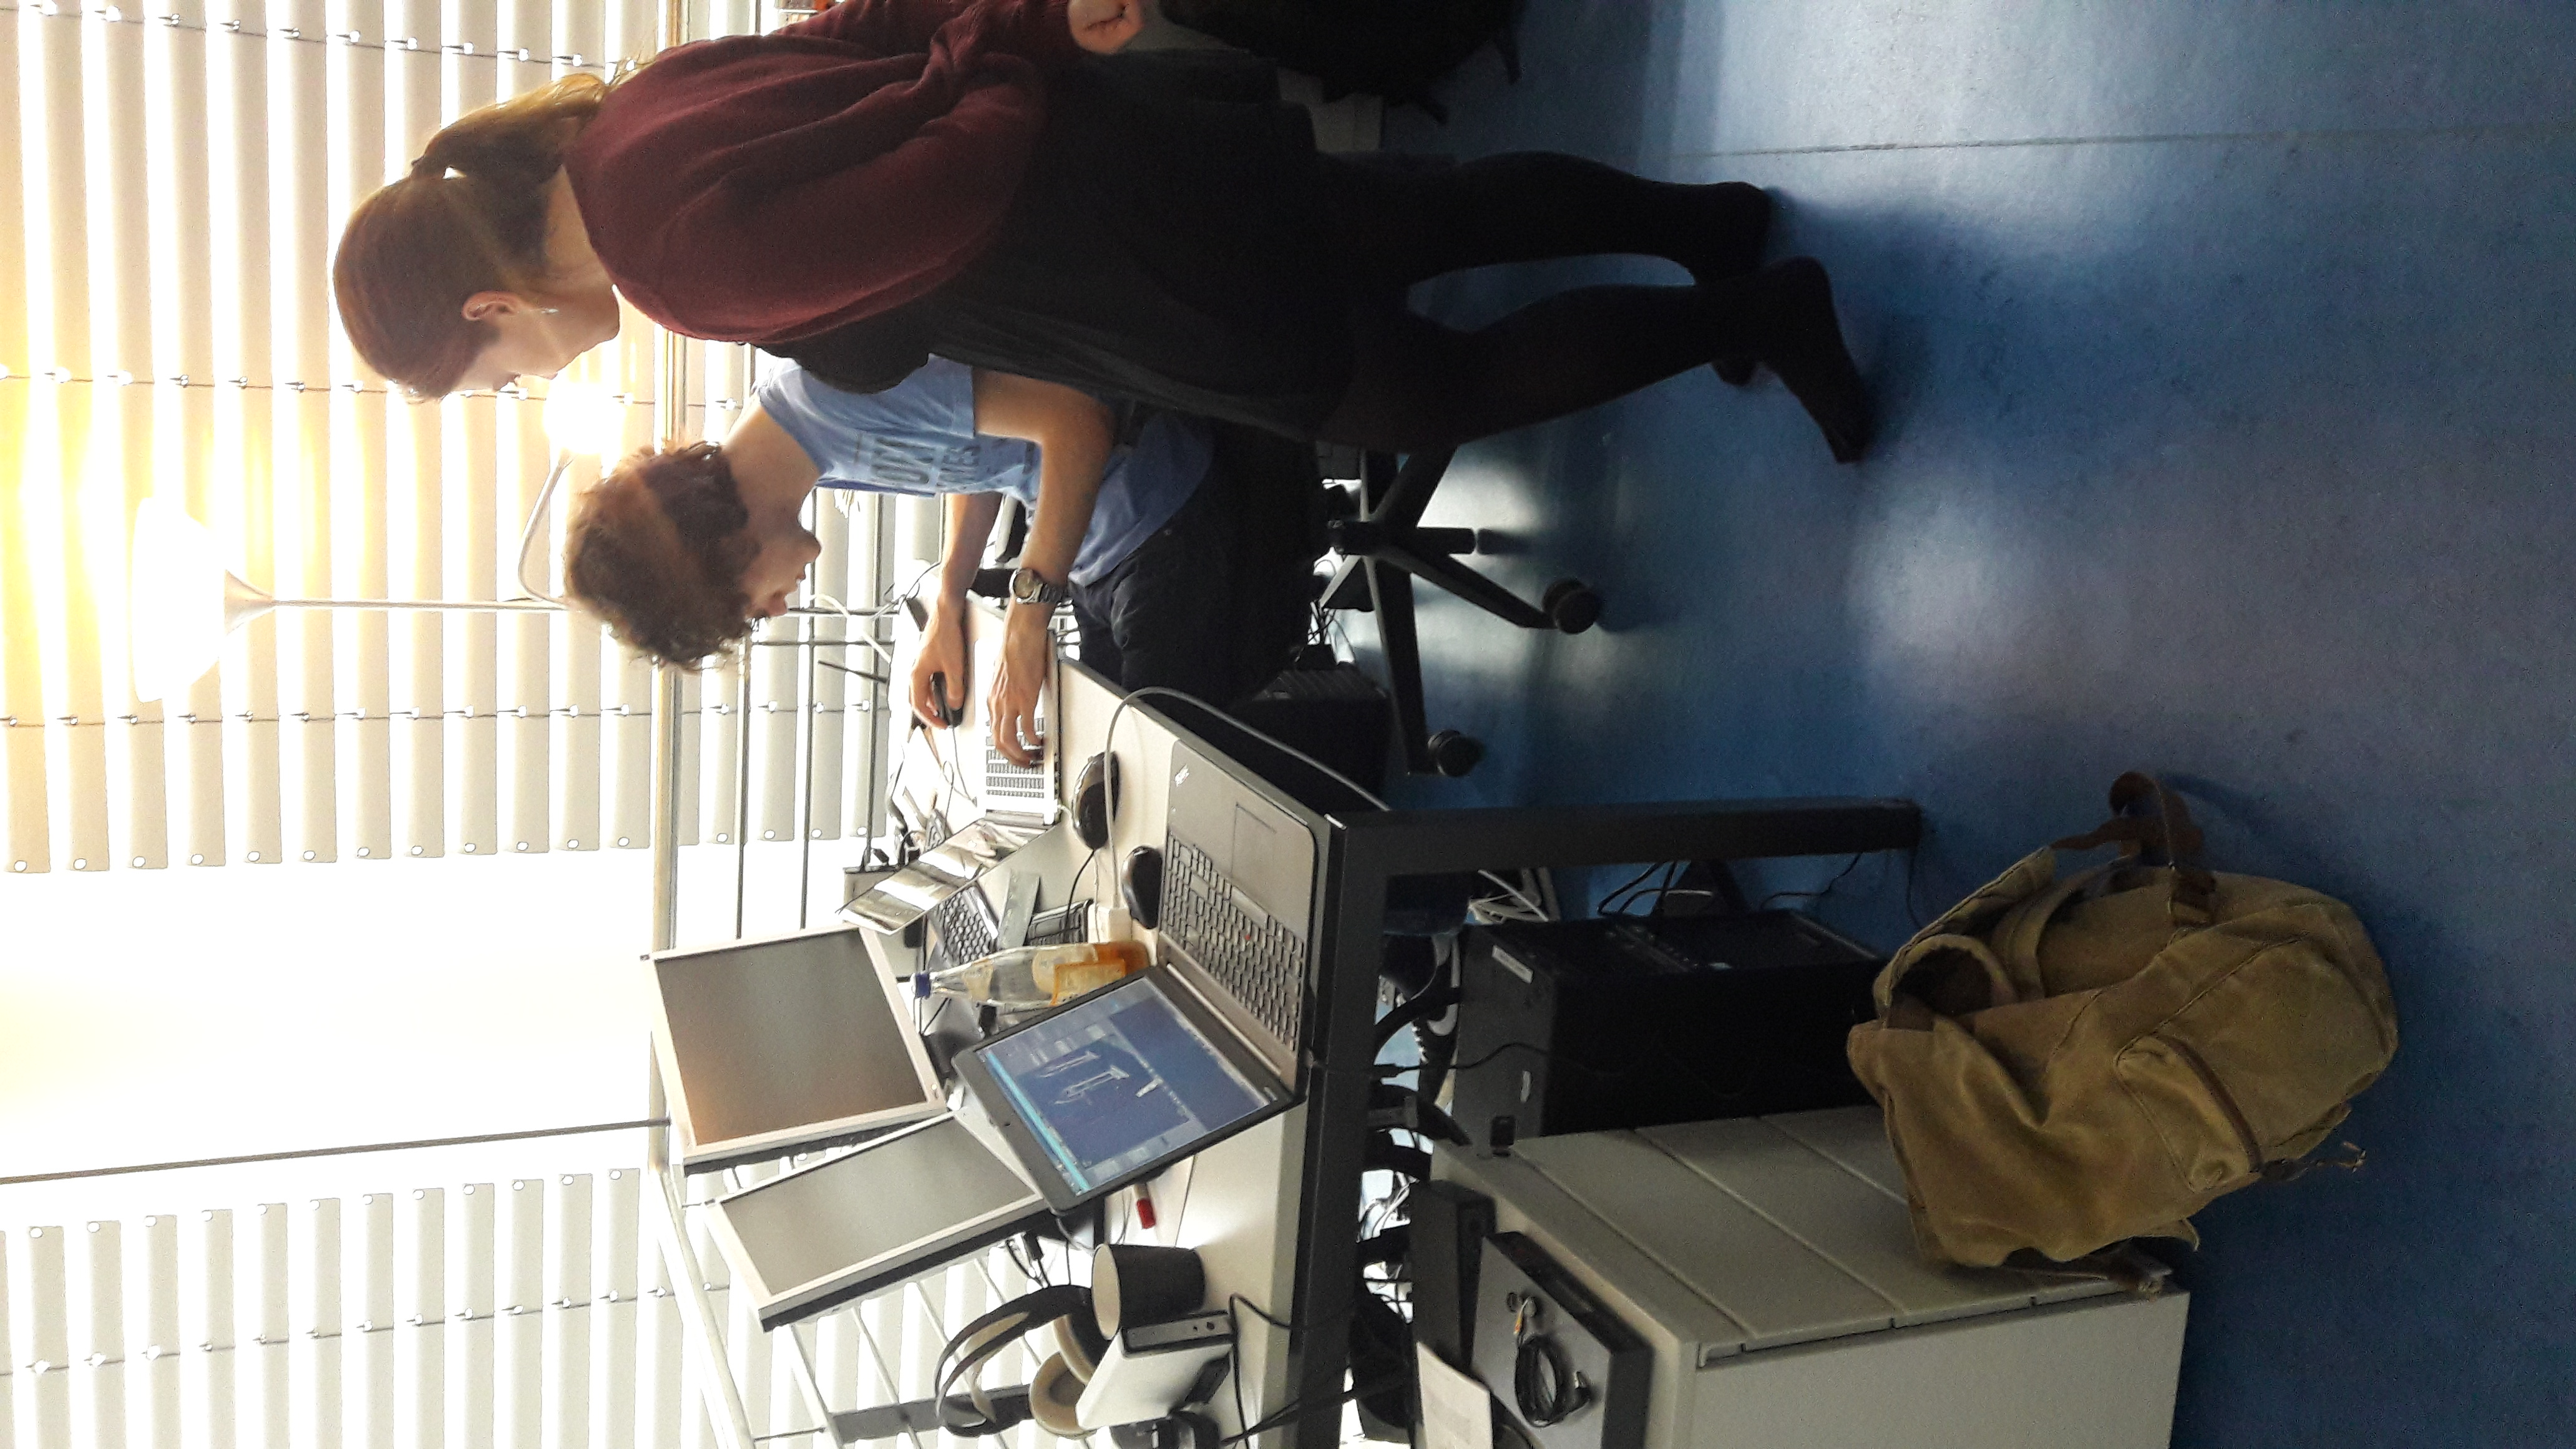
\includegraphics[height=\linewidth, width=\textheight, keepaspectratio, angle=270]{Bilder/20170606_145921.jpg}
			\caption{Problemlösung in Unreal}
			\label{img:porblemloesung}
		\end{figure}

\newpage
		Die Welt war zuerst als recht große Welt geplant, in der man sich frei bewegen kann. Hier sollte man sich viele verschiedene interessante Dinge angucken können und frei durch die Gegend laufen. Hierbei stießen wir jedoch auf das Problem, dass verschiedene Versuchspersonen verschiedene Wege gehen würden und somit unterschiedliche Dinge erleben und manche Szenarien vielleicht sogar komplett auslassen würden. Um dies zu verhindern, kam uns die Idee einer Art Schnitzeljagd. Damit wäre gewährleistet gewesen, dass jeder Versuchsperson ungefähr die gleiche Strecke läuft und das gleiche erlebt wie alle anderen. Jedoch stellte sich auch das als nicht sehr praktikabel heraus. Wir benötigten ein Mapdesign, in dem jede Versuchsperson die gleiche Strecke läuft und das gleiche erlebt.

		So kamen wir darauf, die Versuchspersonen auf einem Gehweg entlanglaufen zu lassen, auf dem es keine betretbaren Abzweigungen gibt und jeder an mehreren Ampeln für eine vordefinierte Zeit warten muss. 
		
		Während des gesamten Designprozesses kam es immer wieder zu Schwierigkeiten und Problemen.
		
		\subsubsection{Blender}
			Blender ist ein sehr komplexes und umfangreiches Programm, dementsprechend hatte jeder von uns eine längere Einarbeitungsphase. Bei kleineren Problemen haben wir uns gegenseitig viel helfen können und unser angesammeltes Wissen ausgetauscht. Die größten Probleme entstanden hauptsächlich nach dem Import in die Unreal Engine. 

			Ein Problem war, dass bei einigen Objekten die Textur nicht korrekt dargestellt wurde oder Objekte teilweise durchsichtig waren. Bewegt man die Kamera in der Unreal Engine in ein Objekt hinein, so sollte man von innen nach außen durch die Objektoberflächen hindurch gucken können. Die Teile, die von außen durchsichtig waren, waren von innen jedoch sichtbar. Somit war das Problem, dass die Objekte teilweise \"auf links gekrempelt\" waren. Mit Hilfe des Anzeigens der Normalen in Blender ließen sich diese Flächen aber leicht aufspüren und umdrehen bzw. die Normale(n) invertieren.
			
			Größere Probleme hatten wir auch bei den Texturen. Die Bearbeitungs-Ansicht (Texture) in Blender entsprach nicht immer der in Blender gerenderten Ansicht (Rendered) und auch nicht der in der Unreal Engine angezeigten Ansicht. Somit hatten wir für ein Objekt teilweise drei verschiedene Ansichten der Textur. Am meisten Probleme machten die Häuser, wohingegen andere Objekte wie der American Store völlig problemlos funktionierten. Gerade bei den Häusern haben wir die Materials, in denen die Texturen enthalten sind, in der Unreal Engine noch stark nachträglich bearbeitet.
			Generell wurden nahezu alle Materials in der Unreal Engine nochmal editiert, da Einstellungen wie Specular Lightning oder Spiegelungen nicht von der Engine übernommen wurden.
			
			Ein zentrales Problem war, dass jegliche von uns erstellten Objekte nach eine Build des Lightnings komplett schwarz waren. Nach einiger Recherche stellte sich heraus, dass alle in der Unreal Engine verwendeten Objekte zwei UV-Maps benötigen. Die zweite ist notwendig für das korrekte Darstellen des Lightning und ist, zumindest bei statischen Objekten, zwingend notwendig. Sich bewegende Objekte wie beispielsweise die Autos werden anders gerendert und benötigen diese zweite UV-Map nicht. 
		
		\subsubsection{Unreal Engine}
			Gestartet haben wir unser Projekt mit der VR-Vorlage von Unreal. Mit der Fertigstellung der ersten Objekte fingen wir an die Welt zu bauen. Eine anfängliche Herausforderung war die Skalierung, da man sich in einer fast leeren Welt kaum an etwas orientieren kann. Nach einiger Recherche haben wir eine Skalierung festgelegt und ein großes Schachbrett mit $1m^{2}$ großen Feldern als Orientierung unter die Map gesetzt. Mit dessen Hilfe haben wir die Straßen und Gehwege platziert. Weiter ging es mit Häusern und Gärten, bis wir schließlich die letzten Details wie Mülleimer, Laternen und Bäume gesetzt hatten. 
			
			Eine Herausforderung stellte unter anderem auch die Logik in unserer Welt da. Die Teleporter und die Ampelschaltung waren die aufwendigsten Sachen, die wir in Blueprints umgesetzt haben. Es hat einige Zeit der Fehlersuche und Fehlerbehebung gegeben, bevor alles funktionierte. Das Fahren der Autos wurde ebenfalls in der Unreal Engine programmiert, die Bewegung der Schaukel hingegen in Blender.
			
			Nach einiger Zeit stellten wir auch fest, dass es für die Spiellogik einen erheblichen Unterschied macht, ob man die Welt mit der Oculus Rift durchläuft, oder \"auf dem Bildschirm\". Beispielsweise wird eine Triggerbox, die man betritt oder verlässt, normalerweise nur einmal getriggert. Beim Betreten/Verlassen mit VR-Ansicht hingegen um die zwanzig mal.
		
		\subsubsection{Hardware \& Software}
			Allerlei Hardware hat, gerade am Anfang, aus uns unbekannten Gründen oftmals nicht so funktioniert wie erwartet. Das hat uns letzten Endes dazu bewegt auf einem neuen Computer eine frische Installation von Windows 10 mit allen aktuellen Updates aufzuspielen. Nachdem alle Treiber und Programme installiert waren und auch alles funktionierte deaktivierten wir jegliche Updates, um eventuelle negative Änderungen am System zu verhindern. 
			
			Außerdem haben wir zeitlich etwa mittig im Designprozesses die anfänglich gewählte VR-Vorlage in Unreal gegen eine 3rd-Person-Vorlage ausgetauscht. Dies vereinfachte das anschließen eines Controllers enorm. Die Einbindung der Virtusphere zur Steuerung stellte sich als zu komplex und zeitaufwendig heraus. 
		
		\subsubsection{Fragebögen und Versuchspersonen}
			Zeitgleich wurden auch die Fragebögen entwickelt und ausformuliert. Es gab drei Stück (A, B und C), einen für vor dem Betreten der VR-Welt, einen für danach und einen nur für uns.
			
			Außerdem gab es einen Intelligenztest. Von anfänglich einem recht umfangreichen sind wir am Ende zu einem sehr kurzen gewechselt, da wir kein exaktes Ergebnis benötigen und den Zeitaufwand für die Versuchspersonen möglichst gering halten wollten.
			
			Zuletzt haben wir eine Einverständniserklärung aufgesetzt, die uns rechtlich absichert und jede Versuchsperson unterschreiben musste.
			
			Zeitgleich mit allen Aufgaben des Designprozesses haben wir nach Versuchspersonen gesucht. Hierzu formulierten wir einen Anzeigentext und veröffentlichten ihn teilweise mehrfach auf dem schwarzen Brett bei bremen.de, eBay Kleinanzeigen und dem schwarzen Brett in Stud.IP. Zusätzlich fragten wir in unserem Bekanntenkreis herum. 
			
			Auf Grund von technischen Schwierigkeiten mussten wir den Start der Versuchsdurchführung einige Male verschieben und mit betroffenen Versuchspersonen einen alternativen Termin absprechen. 
		
	\subsection{Versuchsdurchführung} % Daniel
		Für die Versuchsdurchführung benutzten wir meistens zwei Räume. Ein Raum war für den VR-Teil des Experiments und einer für die Fragebögen und Messungen davor und danach. Im Flur vor den Räumen war ein Wartebereich mit Sofas, Knabbersachen und Getränken. 
		
		In der Zeit der Versuchsdurchführung waren wir nicht alle gleichzeitig anwesend, sondern immer nur ein im Voraus festgelegtes Team. Es gab eine feste Routine, wie wir mit den Probanden umgehen und was wir ihnen sagen oder auch nicht sagen. 
		
	\subsection{Auswertung} % Marvin
	
		%Auswertung
		Das Projekt abschließend folgte nach dem 26.03.2017, dem letzten Tag der Versuchsdurchführung, die Auswertung unserer Ergebnisse.
		Zunächst mussten wir auch in dieser Phase einige zusätzliche Recherche, vor allem zu mathematischen Verfahren für statistische Auswertung, betreiben. Ebenfalls sehr wichtig waren für uns die genauen Richtlinien zur Veröffentlichung eines wissenschaftlichen Papers. Hierzu erhalten wir ein maßgebendes Buch von unseren Dozenten. Wir unterteilten den Inhalt des Papers und dieses Berichts und teilten diese untereinander auf.\\
		Danach begannen wir zunächst damit sämtliche Ergebnisse zu digitalisieren.\\
\\

\section{Versuchsaufbau und Durchführung}
	\todo[inline]{Autor: Nizan}
	\subsection{Probanden}
Für die Durchführung des Experiments haben wir Probanden benötigt, die als Versuchspersonen (Abkürzung VP) für die Untersuchung und Überprüfung unserer Forschungsfrage dienen. 
Die Versuchspersonen waren bezüglich der experimentellen Hypothese unwissend und unterschrieben vor der Teilnahme eine schriftliche Einverständniserklärung mit allen Risiken und Datenschutz-rechtlichen Informationen. Alle Probanden haben freiwillig am Experiment teilgenommen und wurden nicht entschädigt. 
\par

\subsubsection{Demografische Angaben}

Bei der Suche nach Probanden haben wir uns auf Probanden im Alter von minimal 18 Jahren und maximal 80 Jahren beschränkt, da die Zeitwahrnehmung von Jungendlichen langsamer ist als die von Erwachsenen. Der Grund: Je mehr Neues und Emotionales man erlebt, desto mehr prägt sich im Gedächtnis ein; und desto länger wirkt ein Zeitraum im Nachhinein. Das ergab die Studie ?Age effects in perception of time? von Marc Wittmann und Sandra Lehnhoff aus dem Jahre 2005. Weshalb wir ausschließlich Erwachsene Probanden gesucht haben, die über dem Zeitraum der ?erste Male erleben? hinaus sind. Der Mittelwert aller Probanden liegt bei 31 Jahren, ob diese bereits vorher in einer VR waren, haben wir nicht berücksichtigt. \\

Insgesamt wurden 48 gültige Ergebnisse für die Auswertung benötigt, weshalb wir 50 Probanden eingeladen haben um am Experiment teilzunehmen, für mögliche Ausfälle, die auch aufgetreten sind. \\

Die Verteilung der Geschlechter haben wir offen gelassen, da in dem Ausmaß unseres Experiments keine signifikanten Unterschiede zustande gekommen wären, das gilt auch für den Bildungsstand und die Rasse der Probanden. Die Sprachkenntnisse waren uns dennoch wichtig, aufgrund des Mehrfach-Wortschatz Intelligenztests der auf guten Deutschkenntnissen basiert und wir die selben Voraussetzungen bei allen Versuchspersonen gewährleisten wollten. Weitere Voraussetzungen waren eine gute oder auf normal korrigierte Sehkraft durch eine Brille oder Kontaktlinsen und normales Farbsehen. Außerdem haben wir Versuchspersonen mit Gehirnschäden oder psychischen Erkrankungen vom Experiment ausgeschlossen, um mögliche Störvariablen zu verhindern. 


\subsubsection{Probanden Suche} 

Um die Probanden Suche hat sich das Organisation Team gekümmert. Es wurde eine Projekt E-Mail Adresse erstellt, für die Kommunikation und Interaktion zwischen Versuchsleitern und Versuchspersonen. Die Suche verlief auf drei unterschiedlichen Wegen: (1) Bekannte anwerben, (2) Flyer Verteilung, (3) Anzeigen auf Sozialen Netzwerken und öffentlichen Portalen veröffentlichen. In vorher eingeteilten sogenannten ?Terminslots?, im Zeitraum von sechs Tagen, wurden die Probanden eigetragen. Die effektivste Methode Probanden zu finden waren Anzeigen auf der Website ?Ebay-Kleinanzeigen? zu schalten. Diese wurden mehrmals in der Woche von neuem geschaltet, sodass eine Großzahl von Menschen die Anzeige lesen konnte, um sich dann bei uns per Mail zu melden. \\

Die zweit erfolgreichste Methode Probanden zu finden war im Bekanntenkreis passende Probanden anzuwerben. Dabei haben wir im Vorhinein die Grenze gesetzt, keine direkten Verwanden, wie Eltern, Geschwister oder Lebenspartner zu nehmen, da sie eventuelles Vorwissen haben, was das Ergebnis verfälschen könnte. \\

Die Methode mit den Flyer hat am schlechtesten funktioniert, da wir die wenigsten Rückmeldung bekommen haben, was uns gezeigt hat, dass diese Methode etwas veraltet ist.

\par

\underline{Anzeigen Text für Ebay Kleinanzeigen und die Flyer:}

\par

Freiwillige Probanden für VR Experiment gesucht

\par

Bist du im Alter zwischen 18 und 80, bist fit und hast Lust mal in eine Virtuelle Welt einzutauchen? Dann bist du genau die richtige Person um an unserem Experiment teilzunehmen! \\

Wir sind eine Gruppe Studenten aus dem Bereich Digitale Medien von der Universität Bremen und führen im Rahmen unseres Bachelor-Projekts eine Untersuchung zur Wahrnehmung in der virtuellen Realität. Mit einer VR Brille schicken wir dich in eine andere Welt in der du verschiedene Szenarien auf dich einwirken lässt.

\par

Wenn du Interesse hast uns bei unserem Experiment zu unterstützen, dann würden wir uns über eine Email von dir freuen. Nenne uns bitte in deiner Nachricht deinen Namen, Alter, Geschlecht sowie die Tage an denen du zur Verfügung stehst für das VR Experiment - an folgende Adresse: experiment.sose17@gmail.com \\

Unser Experiment werden wir an diesen 6 Terminen durchführen: \\

Mo 19., Mi 21., Do 22., Fr 23., Sa 24. und Mo 26. Juni 2017 immer jeweils zwischen 10 und 18 Uhr, 

im Cartesium an der Universität Bremen. Die Dauer wird 30 Minuten bis 45 Minuten betragen.

Wir freuen uns auf hoffentlich zahlreiche Nachrichten!




Das Experiment Projekt Team


\par

\subsubsection {Ethik}

Die Untersuchung menschlichen Verhaltens mit dem Ziel an Forschungsergebnissen zu gelangen, ist immer etwas problematisch. Besonders, wenn die Manipulation im Rahmen eines Experiments die Persönlichkeit eines Menschen langfristig prägen oder beeinflussen könnte. Das zeigte sich uns schon zu Beginn des Projekts, bei der Frage zum Hauptthema des Experiments. Dabei haben wir unbewusst Themen verworfen, aufgrund der ethischen Moralfrage. Obwohl einige Vorschläge wirklich interessant waren, hat uns unser gesundes ?moralisches Ich? gesagt, dass wir diese Ideen als Experiment keinem Probanden zumuten können. Diese hätten Grenzen überschritten, deren Folgen wir nicht verantworten wollten. Auch wenn es anfänglich unbewusst geschah und wir uns erst später mit der Frage ethischen Vertretbarkeit beschäftigten, haben wir uns stets an die  moralischen Richtlinien gehalten. Die hohe Nachfrage der freiwilligen Probanden hat uns gezeigt, dass uns der Spagat zwischen Ethik und einem Experiment  das menschliches Verhalten testet, gut gelungen ist. Uns war wichtig die Sicherheit der Probanden zu gewährleisten, weshalb sie weitestgehend über Zweck und Ablauf des Verfahrens sowie über die vorhersehbaren Unannehmlichkeiten und Risiken vorab informiert wurden. Es wurde vor der Teilnahme eine schriftliche Einverständniserklärung unterschrieben, womit die Probanden die persönliche Verantwortung übernahmen und somit auch die Risiken in kauf nahmen. Des weiteren haben wir die Versuchspersonen immer ermutigt fragen zu stellen, wenn welche offen waren, um Zweifel oder Missverständnisse zu vermeiden. Zuletzt werde alle Ergebnisse und untersuchten Daten streng vertraulich behandelt und anonymisiert nach den allgemeinen Datenschutzrichtlinien.


\subsection {Apparaturen}

Zwei Räume wurden für die Durchführungen des Experiments genutzt und von uns ausgerichtet. In Raum 1, haben wir die Fragebögen ausfüllen lassen und die Zeit-Einschätzungs-Tests durchgeführt. Dort stand ein Tisch und auf den sich gegenüberliegenden Seiten zwei Stühle. Auf einem separaten Tisch, hinter dem Stuhl der Versuchsleiter, lagen alle benötigten Unterlagen und Werkzeuge: die Ergebnisse der vergangenen Probanden, der Infrarot-Thermometer [?Braun ThermoScan 7 Infrarot Ohrthermometer IRT6520?] sowie die dazugehörigen Schutzkappen - die nach jedem Durchlauf ausgewechselt wurden, ein iPhone 6 zum stoppen der Zeit und die leeren Fragebögen: (1) Einverständniserklärung, (2) ?Fragebogen B?, (3) ?Fragebogen A?, (4) Mehrfach-Wortschatz-Intelligenztest und (5) ?Fragebogen C? (weitere Erläuterungen unter dem Punkt 5.3.A) Diese haben wir der Reihenfolge nach in Klemmbrettern geordnet und für die Durchläufe mit den nächsten Versuchspersonen vorbereitet. 

In Raum 2 haben wir die praktischen VR-Experimente durchgeführt. Dort stand ein Drehstuhl um sich flexibel in der Welt bewegen und drehen zu können, ein Tisch mit einem LG Computer auf dem  Windows 10 installiert war und zwei Monitore [Fujitsu Siemens P19-1A \& 2. Benq FP222WH] auf denen man die virtuelle Welt sehen und mit Unity bearbeiten konnte. Außerdem war der Raum mit Kopfhörern ausgestattet um äußere Geräusche zu minimieren sowie und die Audio und Hintergrundgeräusche in der virtuellen Welt zu demonstrieren; die Occulus DK2 VR-Brille zur Orientierung in der VR und ein XBox-Controller für die Steuerung in der Welt.


\subsection {Experiment Ablauf mit genauen Wortlauten}

Der Zeitraum der Experiment Durchführung lag bei sechs Tagen, in denen jeweils im Durchschnitt 8.3 Versuchspersonen an der Untersuchung teilnahmen. Jeder Durchlauf dauert je nach Proband zwischen 25 Minuten bis 40 Minuten.

\par

Der Ablauf des Experiments bestand aus drei Teilen. Der theoretische Teil vor der VR, der praktische Teil in der VR, und der theoretische Teil nach der VR. Die Messmethode war aussagekräftig, da alle Durchläufe sowie die dazugehörigen Erklärungen bei allen Probanden exakt gleich stattgefunden haben.

\par

\underline{Teil 1.:}

Jeden Durchgang haben wir mit einer Einweisung durch die Räumlichkeiten begonnen. Der erste Teil, der theoretische Teil des Experiments findet in unserem Befragungsraum, ?Raum 1? statt. Es sind immer zwei Versuchsleiter (VL) die den ersten Teil des Versuchs durchführen und dem Probanden gegenüber am Tisch sitzen. Die Arbeit wird geteilt, dass einer VL den Ablauf leitet und der zweite VL die Ergebnisse notiert und auf Fehler achtet. Alle Ergebnisse der Zeiteinschätzungen und die Körpertemperatur werden von dem VL auf dem vorgedruckten ?Fragebogen B? notiert. Die Versuchsperson bekommt keine Einsicht auf ihre Ergebnisse, alle Daten werden verdeckt aufgeschrieben.

\par

Wir händigen dem Proband eine Einverständniserklärung die er unterschreiben muss:

?Als erstes bekommen Sie eine Einverständniserklärung
 zur freiwilligen Teilnahme am Experiment, die sie unterschreiben müssen. Bitte lesen Sie diese gründlich durch. Sollten Sie Fragen haben, werden wir diese gerne beantworten.?

\par

Als nächstes wird ein Zeit-Einschätzungs-Test durchgeführt, in dem der Proband 40 Sekunden einschätzen soll, ohne Hilfsmittel und ohne sich zu unterhalten: \\

?Wir werden nun einen Zeit-Einschätzungs-Test durchführen, indem Sie 40 Sekunden einschätzen sollen. Dabei dürfen Sie sich nicht unterhalten und sollten Sie eine Armbanduhr tragen, bitten wir Sie diese abzunehmen. Bei ?Los? geht es los und wenn Sie das Gefühl haben, dass 40 Sekunden vergangen sind, sagen Sie bitte ?Stop??. Das Ergebnis wird von einem VL notiert.

\par

Das Ergebnis wird von einem der anwesenden VL anhand einer Stoppuhr gemessen und auf dem ?Fragebogen B? erfasst. Der Proband bekommt den ?Fragebogen A? ausgehändigt:

,,Wir bitten Sie diesen Fragebogen einmal auszufüllen? \\

Dort sollen folgende Informationen angegeben werden: (1) ob die zu testende Person unter Drogeneinfluss steht, (2) wie der akute müdigkeitswert ist, (3) ob und an welchen Gehirnschäden oder psychischen Erkrankungen der Proband leidet , (4) welche die Muttersprache der Versuchsperson ist und ob die VP noch Lust hat am Experiment teilzunehmen. Wird das Kästchen mit ?Ja? beantwortet, geht es weiter mit den Tests.

\par

Daraufhin wird der ?Mehrfachwahl-Wortschatz-Intelligenztest? (MWT-B) durchgeführt (weitere Erläuterungen bei 5.3.B). 

\par

?Sie sehen hier mehrere Reihen mit Wörtern. In jeder Reihe steht höchstens ein Wort, das Ihnen vielleicht bekannt ist. Wenn Sie es gefunden haben, streichen Sie es bitte durch. \\

Es  gibt keine zeitliche Begrenzung also können Sie sich ruhig Zeit lassen. Sollten Sie ein Wort nicht kennen, dann raten Sie bitte.? Der ausgefüllte Test wird von den VL entgegengenommen und ein erneuter Zeit-Einschätzungs-Test wird durchgeführt. 

\par

?Wir werden nun erneut einen Zeit-Einschätzungs-Test durchführen, indem Sie 40 Sekunden einschätzen sollen. Dieses Mal werden wir uns mit Ihnen währenddessen unterhalten. Sie dürfen sich und uns gerne unterbrechen, wenn Sie das Gefühl haben, die 40 Sekunden sind vorüber.? Das Ergebnis wird von einem VL notiert.

\par

Anschließend messen wir die Körpertemperatur am Ohr des Probanden, anhand unseres Infrarot-Thermometers. ?Wir werden nun Ihre Körpertemperatur mit diesem Infrarot Thermometer messen.? Ein neuer Aufsatz wird auf den Kopf des Thermometers gesetzt und dem Probanden ins Ohr gehalten ?Achtung, nicht erschrecken?. Das Ergebnis wird von einem VL notiert.

\par

Danach führen wir einen stummen 30 Sekunden Zeit-Einschätzungs-Test. ?Es wird nun erneut einen Zeit-Einschätzungs-Test durchgeführt, diesmal sollen Sie lediglich 30 Sekunden einschätzen ohne sich zu unterhalten. Und Los!?

\par

\underline{Teil 2.:} 

Der Proband wird in den isolierten und Schallgeschützen ?Raum 2? geführt, wo der praktische Teil des Experiment stattfindet. Dort warten die zwei Versuchsleiter von der VR. Währenddessen werten die ersten beiden VL den Intelligenztest aus.  \\

Der Proband bekommt folgende Anweisung: ?Nehmen Sie bitte hier auf dem Drehstuhl platz. Sie kommen jetzt in unsere virtuelle Welt. Bitte halten Sie sich an die allgemeinen Verkehrsregeln und prägen Sie sich die Umgebung ein.? \\

Der Proband setzt sich, bekommt die VR-Brille aufgesetzt und den Xbox Controller in die Hand.

?Die Fortbewegung in der virtuellen Welt wird mittels eines Xbox-Controllers kontrolliert. Mit der rechten Taste können Sie die Ausrichtung der Kamera ändern, dies tun Sie am besten wenn Sie an eine Straßenecke gelangen. Ansonsten schauen Sie sich lieber mit der Brille um. Mit der linken Taste können Sie Vorwärts und Rückwärts gehen, sie dürfen selbst entscheiden wie schnell oder langsam Sie gehen und sich sonst frei bewegen. Sie können auch gerne zwischendurch stehen bleiben und sich umschauen wenn Sie wollen.? Der Proband darf die Steuerung testen, danach werden ihm vom VL die Kopfhörer aufgesetzt und der Durchlauf in der VR beginnt. 

\par

Zu Beginn des VR Experiments wird die Zeit von einem Versuchsleiter gestoppt, solange wie der Proband benötigt um die gesamte Strecke der vier Szenarien zu durchlaufen. Erfasst wird die Zeit vom Zeitpunkt des los Laufens bis zur Ankunft am Schild ?Road Closed?. Die vier Szenarien bilden zusammen die virtuelle Welt und bestehen aus insgesamt vier Ampelphasen. Diese sind visuell und auditiv einer realen Welt nachgebaut mit Wegen, Straßenverkehr, Autolärm, Menschen, Häuser und Bäumen. An jeder Ampelphase gibt es einen manipulierten Faktor, den Zeitgeber, der die Zeitwahrnehmung beeinflusst. Immer zwei der Szenarien gleichen sich optisch, mit dem Unterschied, dass den Gegenteiligen Zeitgeber haben. Ein schneller und ein langsamer. \\

Ampelphase an einem LKW - schnelles Ticken, \\

Ampel mit Vogel und Menschen - langsames Ticken, \\

Ampel neben einem schaukelndem Kind mit rosa Shirt - schnelles schaukeln, \\

Ampel mit Heißluftballon-Plakat bei einem schaukelndem Kind mit grünem Shirt - langsames Schaukeln. 

\par

Die Wartezeit an den Ampeln ist von uns vorgegeben und kann nicht frühzeitig übersprungen werden. Der Proband durchläuft die virtuelle Welt ein mal, ohne Pausen in seinem eigenen Tempo. Die Versuchsleiter beobachten das Verhalten des Probanden in der VR mittels von Bildschirmen und können eingreifen, sollte etwas schiefgehen. Nach Beendigung des Laufs, wird dem Probanden die Brille sowie die Kopfhörer wieder abgesetzt und dieser begibt sich zurück in ?Raum 1?, für den letzten Theorieteil.

\par

\underline{Teil 3.:}

Der Proband nimmt erneut platz am Tisch, gegenüber von den Versuchsleitern. 

Es werden 40 Sekunden ohne Unterhaltung abgeschätzt und vom Versuchsleiter notiert. Die Anweisungen in Teil 3., bleiben die gleichen wie in Teil 1. \\

Der Proband erhält den ?Fragebogen C?, den dieser mit diesen Informationen ausfüllen soll:  (1) die geschätzte Dauer von den einzelnen Szenarien (2), die besten und schlechtesten empfundenen Szenarien, (3) die empfundene Dauer in der virtuellen Welt, (4) den eigens empfundenen Spaßfaktor, (5) auffallende Besonderheiten in der virtuellen Welt und (6) eine Einschätzung worum es in dem Experiment ging.  \\

Ein erneuter Zeit-Einschätzungs-Test wird durchgeführt, in dem die Versuchsperson 40 Sekunden abschätzen und sich gleichzeitig mit einem der Versuchsleiter unterhalten soll. Die Ergebnisse werden von den Versuchsleitern notiert. Zum Schluss findet ein 30 Sekunden Zeit-Einschätzungs-Test ohne reden statt. Das Experiment wird danach beendet. Der Proband darf anschließend seine Zeit-Einschätzungs-Ergebnisse erfahren sowie das Ergebnis vom Intelligenztest. Zum Schluss wird der Proband verabschiedet und der nächste Proband vom Treffpunkt abgeholt.

\subsubsection{Dokumente}

Wir haben uns um unsere Evaluationsdaten zu sammeln für das Verfahren des Fragebogens entschieden. Mit dieser Methode kann man ohne viel Aufwand zu vielen Informationen gelangen, auf die man auch zu späteren Zeitpunkten zurückgreifen kann, da Fragebögen reproduzierbar sind. Sie ermöglichen die Objektivität der Befragung und es wird sichergestellt, dass jede Versuchsperson die exakt selben Fragen beantworten muss. Diese Methode benötigt einen geringeren Personalbedarf gegenüber dem Interview und bietet zudem noch einen Organisationsvorteil, da die Prozedur schneller und flächendeckender abläuft. Durch die Anonymität des Befragten, ist dieser beim ausfüllen des Fragebogens weniger gehemmt und beantwortet die Fragen automatisch ehrlicher aber auch sorgfältiger, weil kein Zeitdruck besteht schnell antworten zu müssen.

\par

\subsubsubsection{Frageb�gen}
Bezug auf ?Fragebogen A?: (links zu den jeweiligen Beweisen müssen noch hinzu) \\

In Fragebogen A wurde der körperliche und psychische Zustand des Probanden abgefragt um mögliche Beeinträchtigungseinflüsse zu kennen. \\

Stehen Sie unter irgendwelchen Drogeneinflüssen oder Medikamenten? \\

Da Drogen jeglicher Art und manche Medikamente die die Wahrnehmung beeinflussen und bei Einfluss dieser Substanzen die Ergebnisse nicht verwendbar wären, haben wir die Probanden nach dieser Information abgefragt. \\

Auf einer Skala von 1 bis 10, wie müde sind Sie? (1 = nicht müde - 10 = sehr müde) \\

Eine sehr hohe Müdigkeit mindert die Konzentrationsfähigkeit. Bei einem Müdigkeitswert ab 8 ist die Messung unter Vorbehalt verwendbar und deshalb auch relevant für unsere End Ergebnisauswertung. \\

Haben Sie Ihnen bekannte Gehirnschäden oder psychische Erkrankungen?\\

Probanden mit Gehirnschäden und psychischen Erkrankungen wärden möglicherweise zu einem verfälschtem Ergebnis führen, weshalb die Probanden nach Erkrankungen abgefragt wurden. \\

Ist Deutsch ihre Muttersprache? Wenn Nein, welche Sprache ist ihre Muttersprache? \\

Die Deutschkenntnisse unserer Probanden waren uns aufgrund des Intelligenztest, der auf der deutschen Sprache basiert wichtig, um alle Probanden auf dem selben Niveau testen zu können.  \\

Möchten Sie das Experiment weiterhin durchführen? \\

Dem Probanden wurde die Möglichkeit gegeben das Experiment vorzeitig zu beenden. 

\par

\underline{Bezug auf ?Fragebogen B?:} 

Dieser Fragebogen diente lediglich den Versuchsleitern zum Zweck die Ergebnisse der Zeiteinschätzungen und Körpertemperatur auf Papier zu bringen, in einer reproduzierbaren und geordneten Form.

\par

\underline{Bezug auf ?Fragebogen C?:}

Sortieren der Szenarien / Ampelphasen vom kürzesten zum längsten mit Sekundenangabe //

Die Messung der Wahrnehmung der einzelnen von uns beeinflussten Szenarien, mittels Gravitationsfaktoren und Auditiven Einflüssen. Durch die Anordnung der Szenarien nach der Zeit zeigt sich wie sehr wir die Wahrnehmung der Versuchspersonen beeinflussen konnten.  Wir haben die sogenannte ?Four alternative forced choice? Methode verwendet und somit die Probanden ?gezwungen? die Szenarien zu sortieren. Was dieser nicht weiß ist, dass jedes Ampelszenario gleich lange gedauert hat (18 Sekunden). So erhoffen wir uns herauszufinden, ob eines der erlebten Szenarien die Zeitwahrnehmung der Probanden rafft oder streckt. \\

Sortieren der Szenarien vom besten zum schlechtesten \\

Wir wollen herausfinden, ob das persönliche optische empfinden der Probanden gegenüber der Umgebung in den Szenarien, die Wahrnehmung der Versuchspersonen beeinflusst hat. \\

Einschätzung der Gesamtdauer in der VR\\

Durch das Multiple Choice Verfahren gab es vier Antwort-Möglichkeiten, was uns eine gute Grundlage zum Vergleichen gab. Damit wollten wir das Empfinden der Probanden testen, ob sie die gesamte Zeit in der VR als länger oder kürzer als die tatsächliche Zeit wahrgenommen haben. Dies ist für uns ein weiterer Interessantes Ergebnis zur Zeitwahrnehmung die wir rausfinden wollen. \\

Hatten Sie Spaß? \\

Die Betrachtung des Spaßfaktors,  da der auch einen erheblichen Einfluss auf die Zeitwahrnehmung nimmt. \\

Besondere Auffälligkeiten \\

Auffälligkeiten die eine Zeitwahrnehmung beeinflussen könnte und ein Platz für die Probanden um ein Kommentar zu hinterlassen. \\

Haben Sie entdeckt was wir mit dem Experiment rausfinden wollten?

Abfragung ob das Experiment zu offensichtlich oder gut genug konzipiert war, dass die Probanden nicht rausgefunden haben was wir testen wollen. 

\par

\subsubsubsection{Intelligenztest}

Basierend auf der Studie ?Zeiterleben in der Tempogesellschaft? vom Autor Pascal Wallisch aus der Uni Chicago, in der beschrieben wird, dass die Intelligenz eines Menschen sein Zeiterleben beeinflusst, haben wir beschlossen einen Intelligenztest in unser Experiment zu integrieren. Bei einem Treffen mit dem Master Psychologie Studenten Till Rachwitz, der sich auf Intelligenztests spezialisiert hat, haben wir verschiedene Methoden kennengelernt, wie man die Intelligenz unserer Probanden testen kann, ohne einen mehrstündigen Test durchführen zu müssen. Dabei sind wir auf den psychologisch anerkannten ?Mehrfach-Wortschatz-Intelligenztest (MWT-B)? in der fünften unveränderten Auflage gestoßen, entwickelt von Siegfried Lehre, veröffentlicht im Jahre 2015, der sehr gut für unser Vorhaben geeignet ist. Dieser bereits langjährig angewandte Test dienst zur Messung des allgemeinen Intelligenzniveaus nach einem einfachen und zuverlässigen Schema. \\

Im MWT-B gilt es aus 37 Wortreihen, bestehend aus jeweils vier erfundenen und einem deutschen Wort, das richtige Wort rauszusuchen und durchzustreichen. Der Schwierigkeitsgrad steigt im Laufe des Tests, es beginnt mit Alltagswörter wie ?Nase? und endet mit sehr raren Worten aus dem deutschen Wortschatz wie ?Purin?. \\

Den MWT-B haben wir in der Testothek an der Psychologischen Abteilung der Uni ausleihen dürfen. Die aktuell verfügbare Leistungsfähigkeit wird anhand dieses Tests mit einem geringen Materialaufwand gemessen. Die einfache Wiederholbarkeit und die schnelle und einfache Durchführung innerhalb von circa 5 Minuten, sind zwei der vielen Vorteile dieses Tests für den Zweck unserer Studie. Zwar spielt die Intelligenz der Probanden in unserem Experiment eine Rolle, jedoch nur eine nebenläufige, sodass wir nicht viel Zeit dafür einplanen wollten wie bei einem Standard Intelligenztest. Ein weiterer Vorteil des MWT-B, ist dass dieser von Personen durchgeführt werden kann, die keine spezielle Ausbildung zur Abnahme von IQ-Tests haben. Des Weiteren ist der Test objektiv, robust und ist weitgehend unabhängig von seelisch-geistigen Störungen. \\

	
\subsubsection{Schwierigkeiten}


\section{Auswertung}
	\todo[inline]{Autor: Nicole \& Svenja}
	Auf die Ergebnisauswertung unseres Experiments wird in der wissenschaftlichen Ausarbeitung genauer eingegangen.

\section{Interpretation}
	\todo[inline]{Autor: Nicole \& Svenja}
	Die darauffolgende Ergebnisinterpretation  wird ebenfalls nur in der wissenschaftlichen Ausarbeitung behandelt.
	
\section{Fazit}
	\todo[inline]{Autor: Chovi}

\subsection{Zusammenfassung}
Wie bereits vorgestellt, lautet unsere Forschungshypothese „Kann man das Zeitempfinden in der Virtuellen Welt durch bestimmte Zeitgeber manipulieren?“.
\par
Um dies zu beantworten haben wir unsere eigene Virtual Reality entwickelt und die von uns ausgewählten auditiven und visuellen Zeitgeber integriert. Von beiden Varianten gab es je zwei Ausführungen, eine langsame von der wir erwartet haben, dass sie zeitdehnend auf die Wahrnehmung des VR-Besuchers wirkt und eine schnelle die zeitverkürzend wirken soll. Unsere VR-Welt bestand aus vier Kreuzungen und jeder von diesen wurde ein Zeitgeber zugeteilt. Während unsere Probanden an der Ampel der jeweiligen Kreuzung warteten, waren sie diesen Zeitgebern ausgesetzt. 
\\
Wie zuvor im Paper beschrieben, wurden vor der VR  die für uns relevanten Daten der Testpersonen aufgenommen, darunter Körpertemperatur, Intelligenz und Müdigkeit. Die Befragung nach der VR bezog sich dann überwiegend auf die Wahrnehmung der eben erwähnten vier Szenarien, mit dem Hauptaugenmerk auf die empfundene Dauer dieser. Mithilfe unserer Ergebnisse, wollten wir herausfinden, ob unsere Hypothese, dass das Zeitempfinden in der VR durch gewisse Zeitgeber gezielt beeinflusst werden kann, belegbar ist.
\subsubsection{Schlüsselergebnisse}
\begin{enumerate}
\item Dass Faktoren wie Alter, Körpertemperatur, Intelligenz und Müdigkeit die Zeiteinschätzung beeinflussen, lässt sich im Rahmen unseres Experiments nicht bestätigen.


\item Es fällt den Probanden leichter, kurze Zeitspannen zu schätzen als längere.
\item Zwischen auditiven und visuellen Zeitgebern ist kein deutlicher Unterschied bezüglich der Wirkung zu verzeichnen.
\item Ablenkungen, hier in Form eines Gespräches, verschlechtern das Ergebnis, da die Zeit als deutlich länger geschätzt wird. 
\item Entsprechend der Ergebnisse unseres Projekts, hat der VR-Besuch unsere Probanden nicht derart beeinflusst, sodass es bemerkenswerte Unterschiede zwischen den Zeitschätzungen vor und nach der VR gibt.
\item Die Hypothese, dass durch schnelle Zeitgeber die Zeit aus Sicht der Probanden entsprechend zügiger vergeht, kann bestätigt werden. Der geschätzte Durchschnittswert liegt  deutlich unter der tatsächlichen Dauer des Szenariums.
\item Die Hypothese, dass durch langsame Zeitgeber die Zeit aus Sicht der Probanden entsprechend langsamer vergeht, kann in dem Sinne bestätigt werden, dass die „Langsamen“ als deutlich länger geschätzt werden, als jene Szenarien mit den schnellen Zeitgebern. Dennoch werden diese nicht länger geschätzt als sie tatsächlich gedauert haben.
\end{enumerate}

\subsection{Der Nutzen der Arbeit}
Verständlicherweise nützt unsere Arbeit Forschenden, die sich mit der VR auseinandersetzen. Die Dimension der VR expandiert und somit wahrscheinlich auch der Zeitraum in dem sich Menschen in der VR aufhalten. Alles wird reeller wirken müssen und Gesetze oder Konzepte, die wir aus unserer Realität kennen, werden dort von Menschenhand gesteuert umgesetzt werden können. Die Zeit wird dabei auch eine Rolle spielen und somit die Zeitgeber. Sinnvoll zu wissen ist es, was hier bei der Umsetzung beachtet werden muss, wie diese Umweltfaktoren auf die VR-Besucher wirken und ob oder welche Unterschiede es zur Wahrnehmung realer Zeitgeber gibt. Die Vorstellung, dass in Zukunft Zeitgeber in der VR derart manipuliert werden können, sodass es dem VR-Besuchenden vorkommt er wäre, beispielsweise mehrere Stunden in der Welt gewesen, wobei es in Echtzeit 15 Minuten waren, ist doch sehr beeindruckend. Man könnte in einer menschgeschaffenen weiteren Dimension, in weniger Zeit mehr erleben.
\par
Unabhängig von der Forschung der VR stellt sich die Funktionsart der menschlichen Zeitwahrnehmung noch als recht mysteriös dar. Diese in einer nicht alltäglichen Umgebung wie der VR zu testen kann neue Perspektiven und Erkenntnisse eröffnen. Ähnlich wie auch die Entwicklung kreativer Computersysteme dazu beiträgt, das Konzept der menschlichen Kreativität besser verstehen zu können.

\subsection{Aufbauende Arbeiten}
\subsubsection{Methodenkritik}
In diesem Teil des Fazits werde ich Schwächen unserer Vorgehensweise aufzeigen.
\par
Die Probanden danach zu bitten nach der VR die Szenarien zeitlich einzuschätzen, erwies sich als problematisch, da dabei eher die Erinnerungsfähigkeit getestet wird. Sie mussten sich im Nachhinein an diesen Zeitraum zurück erinnern, ohne vorher gewusst zu haben, dass sie dem besondere Beachtung schenken sollten. Außerdem, auch wenn auf dem Fragebogen, worauf nach der Länge der Szenarien gefragt wurde, diese kurz beschrieben waren, ist es rückblickend für die Probanden schwer die richtige Zuordnung zu finden. Einige haben sicherlich nicht gewusst von welchem Szenarium die Rede war, sich eventuell zu einer Antwort „gedrängt“ gefühlt und dann geraten, was nicht gerade zur Hochwertigkeit unserer Daten beiträgt. Besser wäre es gewesen während des VR-Aufenthalts, nachdem die Straße vom Probanden überquert wurde, um die Zeitschätzung zu bitten. Hierbei könnte aber auch der Effekt auftreten, dass die Probanden nach der ersten oder zweiten Ampel verstehen worum es geht und dann bei der nächsten Ampel die Sekunden zählen. Das wäre auch nicht optimal, aber eine bessere Option als jenes von uns Umgesetzte.
\par
Auch hätte unsere Welt minimalistischer gestaltet werden sollen, damit unsere Zeitgeber klarer zum Vorschein treten. Alles hätte beispielsweise in dezenten Farben dargestellt werden können und ohne aufwendige Texturen. Nur unsere Zeitgeber, wie z.B. das Kind auf der Schaukel, sollten auffallend inszeniert werden. Zwar wäre dadurch ein noch geringerer Spaßfaktor gegeben, aber die Daten die wir gesammelt hätten wären eindeutiger. Viele Probanden haben sich auf unsere Anmerkung hin, dass sie aufmerksam sein sollten alles Erdenkliche gemerkt. Von den Farben der Dächer und den Texturen der Haustüren bis zu der Garderobe der VR-Passanten. Wir hätten den Testpersonen gegenüber erwähnen können, dass sie wachsam sein sollten wenn sie vor der Ampel stehen, sowohl hörend als auch sehend.
\par
Ein weiteres Manko ist, dass auf dem Fragebogen, auf welchem die Zeitschätzungen eingetragen werden mussten,  die Zeitintervalle von uns ungünstig gewählt waren. Diese betrugen 0-7, 7-15, 15-25, 25-35 und länger als 35 Minuten, stammend aus der Zeit in der wir dachten, wir würden die Verticesphere verwenden. Da dies nicht der Fall war und derart weite Zeitspannen nicht nötig waren, hätten uns kürzere Intervalle bis vielleicht 10 min präzisere Ergebnisse gebracht. In unseren Ergebnissen hat eine klare Mehrheit von 70\% angegeben, sie hätten das Gefühl gehabt von 0-7 Minuten in der Welt gewesen zu sein, was bei der Größe der Welt und der Geschwindigkeit mit der man sich darin bewegen kann, recht vorhersehbar ist und für uns kein Wert von höherem Interesse ist.
\par
Außerdem, wenn bereits der Spaßfaktor gemessen wird, sollte etwas in die VR integriert sein, das auch Spaß bringt. Beispielsweise ein kleines Spiel oder Ähnliches, denn lediglich an der Straße längs zu gehen ist in der Welt vielleicht interessant, bewirkt aber wahrscheinlich nicht so viel spielerisches Vergnügen, sodass der Einfluss auf unsere Ergebnisse groß  genug ist. Auch hatten unsere Probanden das Gefühl ständig um die Ecke und gefühlt im Kreis zu gehen, das mag zwar monoton sein, aber durch diesen Aufbau konnten wir wiederum am besten unsere Umgebung manipulieren.
\par
Hinzuzufügen ist, dass aus theoretischer Sicht der Intelligenztest ausführlicher sein sollte und wir mehr Probanden gebraucht hätten, um genauere Ergebnisse zu erzielen und Unschärfe bei den Messungen zu vermeiden.
Eine andere Form der Umsetzung gestaltete sich jedoch aus zeitlichen Gründen schwieriger.
\subsubsection{Folgearbeiten}
Eine Möglichkeit ist es, den Zeitraum des Aufenthalts zu verlängern und mehrere Zeitgeber zu intergieren. Die Konfrontation der Testpersonen mit diesen kann dann nicht nur in einer Situation, beziehungsweise einem Szenarium erfolgen, sondern während des gesamten Aufenthalts in der VR. Die dargestellte Umwelt spiegelt die jeweilige Geschwindigkeit wieder. Bestenfalls sollte man die Testperson zur Interaktion auffordern, so wie wir es uns auch am Anfang der Ideenfindung vorgestellt haben, bevor wir es aus zeitlicher Begrenzung der Umsetzung vereinfachen mussten. Nach dem Aufenthalt könnte man prüfen, ob der Person die Abläufe in der Realität langsamer erscheinen. Wenn dies der Fall ist, sollte man messen wie lange es dauert bis die Wahrnehmung sich wieder normalisiert und wenn das Know-how besteht, Nachforschungen darüber anstellen welche Strukturen sich Gehirn verändert haben. Dies wäre auch ein weiterer Ansatz menschliche Zeitwahrnehmung zu verstehen.
\\
Außerdem könnte man versuchen, langsame und schnelle Zeitgeber zu  kombinieren, um zu schauen, ob es dabei zur Reizüberflutung und Überforderung kommt oder ob so etwas wie ein „inneres“ natürliches Zeitgefühl durch nicht eindeutige Beeinflussung bestehen bleibt.
\par
Das Gebiet im Gehirn, dass das Empfinden der Zeit reguliert, wurde von den Wissenschaftlern vom Medical College of Wisconsin in Milwaukee und des Veterans Affairs Medical Center in Albuquerque entdeckt. Es handelt sich um die Basalganglien, einer funktionellen Einheit von Kerngebieten im Gehirn, die der Bewegungskoordination dienlich sind. Ginge man davon aus, dass sich die Zeitwahrnehmung durch die VR signifikant verändern lassen könnte, dann wäre es vielleicht möglich Krankhaft falsch funktionierende Zeitwahrnehmung, wie sie etwa bei den Aufmerksamkeitsdefizitsyndrom - Patienten gegeben ist, mit regelmäßigen VR-Besuchen zu behandeln. Unter der Voraussetzung, dass es  möglich ist durch regelmäßigen Aufenthalt in der VR die Struktur der Basalganglien zu beeinflussen, könnten diese Störungen möglicherweise verbessert werden.
\par
Außerdem gibt es da noch das auf unserem aufbauende Projekt von Mert Özenen. Dieses wird einen ähnlichen Ablauf wie unseres haben, nur das zusätzlich Umweltfaktoren, wie z.B. Sonne und Wind, durch entsprechende Beleuchtung und einem Ventilator simuliert werden.

\textit{Die Quellen zu diesem Text sind noch nicht ordnungsgemäß eingefügt, sondern auskommentiert in der Tex-Datei. Dies erfolgt noch in einer Bib-Datei und dann auch in zu erwartender Form.}
%\\Quellen:}
%$https://forum.golem.de/kommentare/mobile-computing/marktforschung-gaming-markt-waechst-weiter-vr-und-ar-haben-potenzial/110719,list.html$
%\\
%$http://blog.zeit.de/teilchen/2015/06/19/warum-uns-die-rueckfahrt-kuerzer-vorkommt/$
%\\
%$https://books.google.de/books?id=825bDAAAQBAJ&pg=PT15&lpg=PT15&dq=zeitwahrnehmung+unerforscht&source=bl&ots=Mw-fdpG9ZL&sig=ZDG7tmSi20wubmYZnpGGv0d9K-w&hl=de&sa=X&ved=0ahUKEwii2O3twZPVAhVJVhQKHcvXDUsQ6AEIJzAA#v=onepage&q=zeitwahrnehmung%20unerforscht&f=false$
%\\
%$https://www.google.de/url?sa=t&rct=j&q=&esrc=s&source=web&cd=10&cad=rja&uact=8&ved=0ahUKEwjVoIy0w5PVAhUGuRQKHcf7BzMQFgh4MAk&url=http%3A%2F%2Fwww.fizyka.umk.pl%2Fpublications%2Fkmk%2F07-Duch-creativity.pdf&usg=AFQjCNFWbYAJULT6wNRbbp9krkfaVRISVQ$
%\\
%$http://www.wissenschaft.de/leben-umwelt/hirnforschung/-/journal_content/56/12054/1218133/Gehirnregionen-f%C3%BCr-das-Zeitgef%C3%BChl-gefunden/$
%\\
%$https://www.volkskrankheit.net/news/kinder-kindererkrankungen/zeitwahrnehmung-durch-adhs$
%\\$https://www.google.de/url?sa=t&rct=j&q=&esrc=s&source=web&cd=10&cad=rja&uact=8&ved=0ahUKEwjVoIy0w5PVAhUGuRQKHcf7BzMQFgh4MAk&url=http%3A%2F%2Fwww.fizyka.umk.pl%2Fpublications%2Fkmk%2F07-Duch-creativity.pdf&usg=AFQjCNFWbYAJULT6wNRbbp9krkfaVRISVQ$


\section{Abschließende Gedanken}
	\todo[inline]{Autor: Jana}
	Wir sind in den verschiedenen Phasen des Projekts auf unterschiedliche Probleme gestoßen, von denen wir viele zeitnah lösen konnten. Allerdings gab es auch schwerwiegendere, deren Lösung für uns nicht gleich oder gar nicht offensichtlich war und die unseren ursprünglichen Zeitplan infolgedessen ungewollt stark beeinflusst haben.\\
	Eines der größten Hindernisse in unserem Projekt waren technische Probleme, die ein Vorankommen sehr stark verzögerten und in einem veränderten Zeitplan resultierten.\\
	Durch die Inkompabilität der Ocolus Rift und dem Computer der Virtusphere konnten wir unser Projekt nicht wie ursprünglich geplant in der Virtusphere stattfinden lassen und mussten auf herkömmliche Controller ausweichen. Diese Umstellung ist sehr ärgerlich, da viel Zeit in die Problemlösung investiert wurde und wir den Probanden letztendlich doch nicht das bieten konnten, mit dem wir sie ursprünglich geworben haben. 
	Weiterhin zu kritisieren wäre eine nicht ganz ideale Arbeitsteilung, wodurch es gerade am Ende zu erheblichem Zeitverzug kam. Insbesondere das sog. \textit{Technikteam}, welches primär für die Erstellung der Blenderobjekte, das Einsetzen und das Animieren der Welt verantwortlich war, hat gleich zu Beginn des Projekts anstehende Aufgaben nicht sinnvoll verteilt. Alle Mitglieder waren gleichermaßen nur mit \textit{aktuellen} Aufgaben beschäftigt. D.h., dass zunächst jeder für die Erstellung von Blenderobjekten verantwortlich waren und so Kapazitäten und Zeit verschwendet wurde, da sich bisher noch keiner besonders gut mit der Software auskannte und sich alle gleichermaßen neu einarbeiten mussten.\\
	Diese Entscheidung mag daraus resultieren, dass wir im Bezug auf diese Art von selbstorganisierter Arbeit sehr unerfahren sind und es dadurch zu Fehleinschätzungen kam.\\
	Im Nachhinein stellen wir weiterhin fest, dass es für das Projekt besser gewesen wäre, hätten wir zu Beginn andere Prioritäten festgelegt. Da die Logik der Welt der Punkt ist, von dem die Ergebnisse abhängen, hätte man sich zuallererst auch mit dieser beschäftigen müssen bzw. rechtzeitig die Personen bestimmen müssen, die die Hauptverantwortung für diese übernehmen.\\
	Auch diese Fehleinschätzung zeigte sich im Nachhinein als kritisch und mag ebenfalls aus unserer Unerfahrenheit stammen.
	Trotz aller Probleme können wir aus unserem Projekt auch Positives ziehen. So z.B. haben sich alle des Technikteams in Blender und zum Teil auch Unreal eingearbeitet und konnten Erfahungen mit diesen Softwares sammeln.\\	
	Besonders freuen wir uns im Nachhinein aber darüber, dass wir trotz teils erheblicher Probleme und Aussichtslosigkeit das Projekt zu Ende bringen konnten und es auch bis zum Schluss mit Ernsthaftigkeit getan haben. Gerade weil wir in der kritischen Phase des Projekt starke Probleme hatten, war die Frustration hoch. Nichtsdestoweniger haben wir anfallenden Probleme kreativ zu lösen versucht (bspw. der Versuch das Experiment auf das Laufband zu verschieben) und gewissenhaft versucht, das Projekt noch irgendwie zu retten anstatt es gleich aufzugeben. Und im Nachhinein stellen wir fest, dass gerade die kritischen Fehler uns, so ärgerlich sie auch sind, geholfen haben zu verstehen, wie Gruppenarbeit besser organisiert wäre bzw. haben wir durch das Experiment gelernt, auf welche Punkte besonders zu achten sind. Diese negativen Erfahrungen sind für uns von Bedeutung, da wir gerade auch durch diese viel gelernt haben.\\ 
Nicht unerwähnt sollen allerdings auch die positiven Erfahungen sein, die wir innherhalb der Gruppe und gerade zum Schluss des Projekts mit den Probanden erfahren konnten. Besonders das Zwischenmenschliche, die Kommunikation und Gruppendynamik bewerten wir als sehr gut und eine Stärke der gesamten Gruppe. 


\section{Appendix} % = Anhang
	\todo[inline]{Autor: Alina}
	Anhang.
	
\vfill %Zum Seitenende Verschieben

\printbibliography

\end{document}
